\chapter{System Architecture of UAV-based LoRa Communication}

\section{Overview of Methodology}
The methodology mainly consists of the deployment of LoRa sensor nodes, integration of LoRa transceivers with UAVs, flight path planning, and data transmission to the network server. The overall workflow is shown in Fig. 3.1. UAVs act as mobile gateways that collect data from multiple ground-based LoRa nodes and forward the aggregated data to the central server through suitable backhaul links.

\begin{figure}[htbp]
\centering
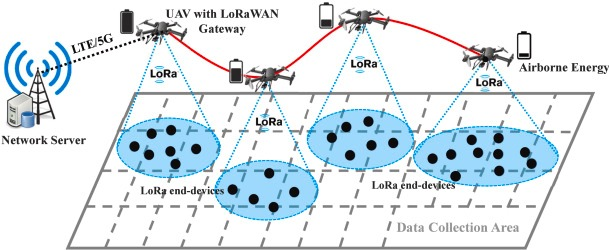
\includegraphics[width=1.1\textwidth,height=.6\textheight]{methodolgy.jpeg}
\caption{Block schematic of the proposed UAV–LoRa communication system} \label{pm}
\end{figure}

\subsection{LoRa Sensor Nodes}
The ground sensor nodes are equipped with LoRa transceivers that operate in the sub-GHz ISM bands (e.g., 433 MHz, 868 MHz, 915 MHz). These nodes are deployed for applications such as environmental monitoring, precision agriculture, or disaster management. Each node consists of a sensing module, a low-power microcontroller, and a LoRa transceiver. The nodes periodically transmit data packets to the UAV-based gateway. Fig. 3.2 illustrates the deployment distribution of sensor nodes.

\begin{figure}[h]
\centering
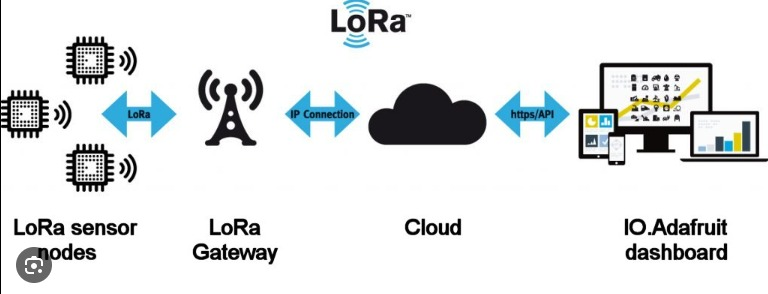
\includegraphics[width=.7\textwidth]{download.jpeg}
\caption{Illustration of LoRa sensor node deployment} \label{pm}
\end{figure}

\begin{figure}[h]
\centering
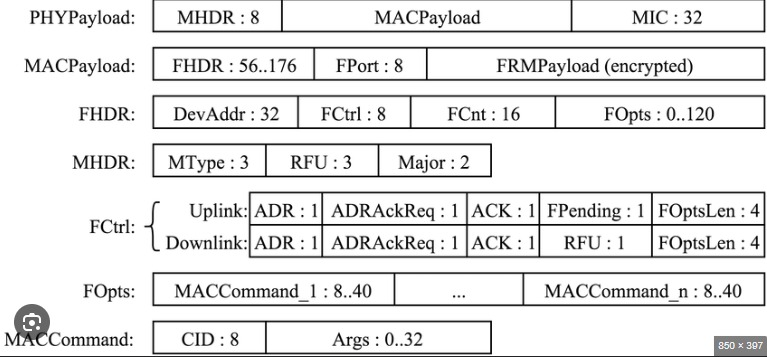
\includegraphics[width=.9\textwidth,height=.6\textheight]{arch.jpeg}
\caption{Example data collected from distributed sensor nodes} \label{pm}
\end{figure}

\paragraph{}
The nodes are typically battery-powered and optimized for long-term operation, transmitting data at low duty cycles. LoRa modulation ensures reliable communication over distances ranging from a few kilometers in urban areas to more than 15 km in rural or line-of-sight conditions. However, node distribution can be irregular, leading to variations in connectivity and link quality, which the UAV helps to overcome.

\subsection{Pre-processing and Data Aggregation}
In UAV–LoRa systems, imbalanced traffic may occur because some nodes transmit data more frequently than others, depending on sensing requirements. Without proper aggregation, this can cause packet collisions or uneven load distribution. The UAV gateway employs data aggregation techniques, buffering incoming packets and forwarding them in batches to reduce network congestion. 

\paragraph{}
Additional strategies such as adaptive data rates (ADR) and duty cycle enforcement help balance communication efficiency. Data pre-processing may also involve compressing payloads, filtering redundant data, and applying error correction codes. The UAV can temporarily store the collected data during flight and later transmit it to the ground station or cloud server when a stable backhaul link (Wi-Fi, 4G, or direct RF link) is available.

\subsection{UAV Gateway Platform}
The UAV acts as a mobile gateway or relay node. It is typically a quadcopter or fixed-wing drone depending on endurance requirements. Fig. 3.3 shows the UAV–LoRa gateway concept. The UAV carries a LoRa transceiver, a flight controller (e.g., ArduPilot/PX4), GPS module, and communication backhaul module.


\subsubsection{LoRa Module Integration}
The LoRa module is interfaced with the UAV’s onboard controller to manage packet reception and forwarding. Parameters such as spreading factor, bandwidth, and coding rate are configured based on application requirements. Higher spreading factors increase communication range but reduce data rates, while lower spreading factors improve throughput at the cost of range.

\subsubsection{Flight Path and Coverage Optimization}
UAVs must follow optimized flight paths to maximize ground node coverage while minimizing energy consumption. Algorithms for path planning consider node density, terrain obstacles, and link quality. Altitude also plays a key role in ensuring line-of-sight communication.

\subsubsection{Data Transmission to Server}
After collecting and aggregating sensor data, the UAV forwards the packets to a central server. This can be achieved using:  
- Direct RF link to a ground base station.  
- Wi-Fi backhaul when within range.  
- Cellular/4G/5G modules for wide-area connectivity.  

\section{Proposed UAV–LoRa System Model}
From prior studies, it is clear that UAV-mounted gateways improve coverage and reliability. In the proposed model, the UAV is equipped with a LoRa transceiver, GPS, flight controller, and communication backhaul. The architecture consists of three main layers: sensor layer (ground LoRa nodes), UAV relay layer (aerial gateway), and application layer (network server/cloud). Fig. 3.4 shows the proposed system.

\paragraph{}
The UAV dynamically adjusts its flight path and communication parameters to maintain connectivity. Adaptive spreading factor allocation and power control help minimize energy consumption. The system also employs buffering and retransmission strategies to reduce packet loss during intermittent connectivity.

\paragraph{}
An optimization algorithm governs UAV altitude and trajectory to balance coverage and flight time. Unlike static LoRa gateways, this mobile gateway approach reduces dead zones and extends network range. The proposed system ensures reliable, energy-efficient, and scalable wireless communication for real-world IoT applications.

\section{Enhancing Communication Reliability}
Challenges such as interference, bandwidth limitations, and UAV power constraints are addressed using adaptive protocols. Channel hopping techniques reduce interference, while duty-cycle-aware scheduling ensures fair resource allocation. UAV battery efficiency is improved by lightweight LoRa hardware and optimized flight trajectories. Future improvements may include swarm UAV coordination, where multiple drones collaborate to provide seamless communication coverage.\cite{inbook}\cite{inproceedings}
